Stimfit was originally written by Peter Jonas, University of Freiburg, in the early 1990s. It was primarily designed to analyse the kinetics of evoked excitatory postsynaptic currents (EPSCs; \citetext{Jonas93}). The name ``Stimfit'' was chosen because the program allowed to \textit{fit} exponential functions to the decay of EPSCs evoked by extracellular \textit{stim}ulation\footnote{Be reassured that I would choose a different name if I had to sell the program.}. The program was written in Borland Pascal, running under DOS and entirely controlled using keyboard shortcuts (Fig. \ref{stimfitdos}). The user interface was similar to a digital oscilloscope, with vertical cursors defining measurement windows for baseline calculation, peak detection and curve fitting. This allowed to analyse data with surprising efficiency once the keyboard shortcuts were mastered. However, the Borland Pascal compiler imposed some significant restrictions which became apparent with increasing data size and computing power: for instance, arrays were not allowed to be longer than 10\textsuperscript{4} elements, and faster processors had to be artificially slowed down to avoid runtime errors.
\begin{myfigure}[ht]
    \begin{center}
      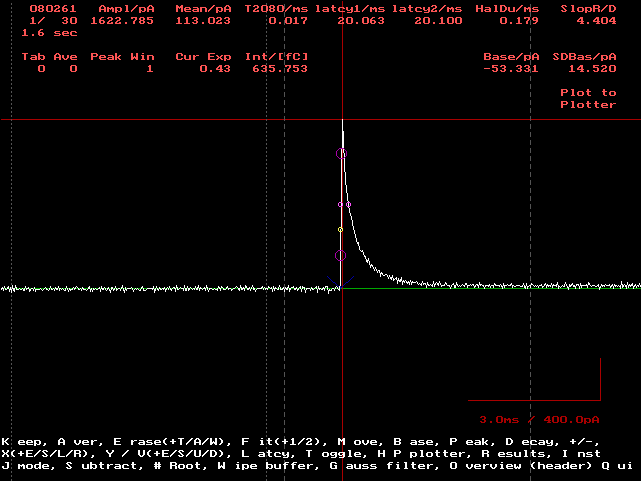
\includegraphics[scale = 0.5]{./img/stimfit_dos.eps}
    \end{center}
    \caption{The original Stimfit for DOS.}
    \label{stimfitdos}
\end{myfigure}

When I converted the original Pascal program to C/C++, I rewrote the code almost entirely from scratch. Only the algorithms to calculate latencies, rise times, half durations and slopes are direct translations of the original Pascal code. By contrast, I tried to preserve the user interface as far as possible. Therefore, the program only poorly adheres to common conventions for graphical user interfaces: For instance, clicking the right mouse button will usually set a cursor position rather than popping up a context menu.

A number of people have contributed to the program: First, I would like to thank Peter Jonas for the original Stimfit code. Josef Bischofberger has added some functions to the DOS version which I have adopted. Bill Anderson has made helpful suggestions concerning the user interface and provided some very large files that have been recorded with his free program \href{http://www.winltp.com}{WinLTP}\footnote{\url{http://www.winltp.com}}. A large amount of helpful comments and bug reports were filed by Emmanuel Eggermann and Daniel Doischer. The Levenberg-Marquardt algorithm used for curve fitting was implemented by  \href{http://www.ics.forth.gr/~lourakis/levmar/}{Manolis Lourakis}\footnote{\url{http://www.ics.forth.gr/~lourakis/levmar/}}.
